\section{Przypadek Testowy 1 - Algorytm genetyczny - zależność PRD od ilości iteracji}
  \subsection{Cel:}
    W tej części zostaną ze sobą porównane PRD rozwiązania algorytmu genetycznego w zależności od liczby iteracji.
    \subsection{Założenia:}
    Do badania tego przypadku została wykorzystana instancja \textbf{berlin52.tsp}. Dodatkowo współczynnik mutacji został ustalony na 0.15, współczynnik selekcji na 0.95. Ponad to wielkość populacji została ustalona na {10, 20, 30, 40}. Badane iteracje były z zakresu {1000, 2000, 3000, ... 10000}. Dla każdej wielkości populacji testy zostały przeprowadzone 10 razy.
  \subsection{Wyniki: }
  Poniższe tabele przedstawiają wyniki testów, odchylenie standardowe oraz błęd standardowy. 
  \begin{table}[!ht]
    \centering
    \begin{tabular}{|l|l|l|l|l|}
    \hline
             & 10    & 20    & 30    & 40    \\ \hline
        1000 & 80.47 & 61.66 & 43.67 & 57.52 \\ \hline
        2000 & 62.40 & 48.94 & 39.31 & 45.41 \\ \hline
        3000 & 47.33 & 45.31 & 38.33 & 38.38 \\ \hline
        4000 & 36.40 & 39.02 & 32.11 & 32.29 \\ \hline
        5000 & 49.98 & 34.98 & 30.57 & 25.19 \\ \hline
        6000 & 34.92 & 33.88 & 32.87 & 30.54 \\ \hline
        7000 & 37.85 & 34.57 & 29.66 & 25.77 \\ \hline
        8000 & 39.34 & 34.57 & 25.27 & 27.23 \\ \hline
        9000 & 37.54 & 26.08 & 25.11 & 22.17 \\ \hline
        10000 & 38.83 & 28.65& 24.14 & 22.52 \\ \hline
    \end{tabular}
    \caption{Wyniki to wartości PRD (wyrażone w procętach), uśrednione. }
  \end{table}

  \begin{table}[!ht]
    \centering
    \begin{tabular}{|l|l|l|l|l|}
    \hline
        SD & 10 & 20 & 30 & 40 \\ \hline
        1000 & 13.96 & 11.90 & 9.46 & 18.87 \\ \hline
        2000 & 18.91 & 11.07 & 8.42 & 16.18 \\ \hline
        3000 & 12.87 & 12.22 & 10.20 & 12.82 \\ \hline
        4000 & 15.65 & 16.56 & 9.80 & 10.56 \\ \hline
        5000 & 18.25 & 10.17 & 14.08 & 5.57 \\ \hline
        6000 & 11.27 & 10.79 & 7.59 & 8.99 \\ \hline
        7000 & 11.27 & 15.08 & 10.46 & 8.64 \\ \hline
        8000 & 13.86 & 9.02 & 9.84 & 9.10 \\ \hline
        9000 & 15.78 & 8.49 & 7.34 & 8.81 \\ \hline
        10000 & 17.20 & 9.70 & 8.36 & 7.42 \\ \hline
    \end{tabular}
    \caption{SD - Odchylenie standardowe}
  \end{table}

  \begin{table}[!ht]
    \centering
    \begin{tabular}{|l|l|l|l|l|}
    \hline
        SE & 10 & 20 & 30 & 40 \\ \hline
        1000 & 4.41 & 3.76 & 2.99 & 5.97 \\ \hline
        2000 & 5.98 & 3.50 & 2.66 & 5.12 \\ \hline
        3000 & 4.07 & 3.86 & 3.23 & 4.06 \\ \hline
        4000 & 4.95 & 5.24 & 3.10 & 3.34 \\ \hline
        5000 & 5.77 & 3.22 & 4.45 & 1.76 \\ \hline
        6000 & 3.56 & 3.41 & 2.40 & 2.84 \\ \hline
        7000 & 3.56 & 4.77 & 3.31 & 2.73 \\ \hline
        8000 & 4.38 & 2.85 & 3.11 & 2.88 \\ \hline
        9000 & 4.99 & 2.68 & 2.32 & 2.79 \\ \hline
        10000 & 5.44 & 3.07 & 2.64 & 2.35 \\ \hline
    \end{tabular}
    \caption{SE - Błąd standardowy}
  \end{table}

  Odchylenie standardowe oraz błąd standardowy zostały obliczone według wzorów: \\
    Odchylenie standardowe:
    \[ \sigma = \sqrt{\frac{\sum_{n = 1}^{10}(\bar{x} - x_n)^2}{10}} \]
    Błąd standardowe:
    \[ \sigma_{\bar{x}} = \frac{\sigma}{\sqrt{10}} \]

  \subsection{Wykresy: }
    \begin{figure}[H]
      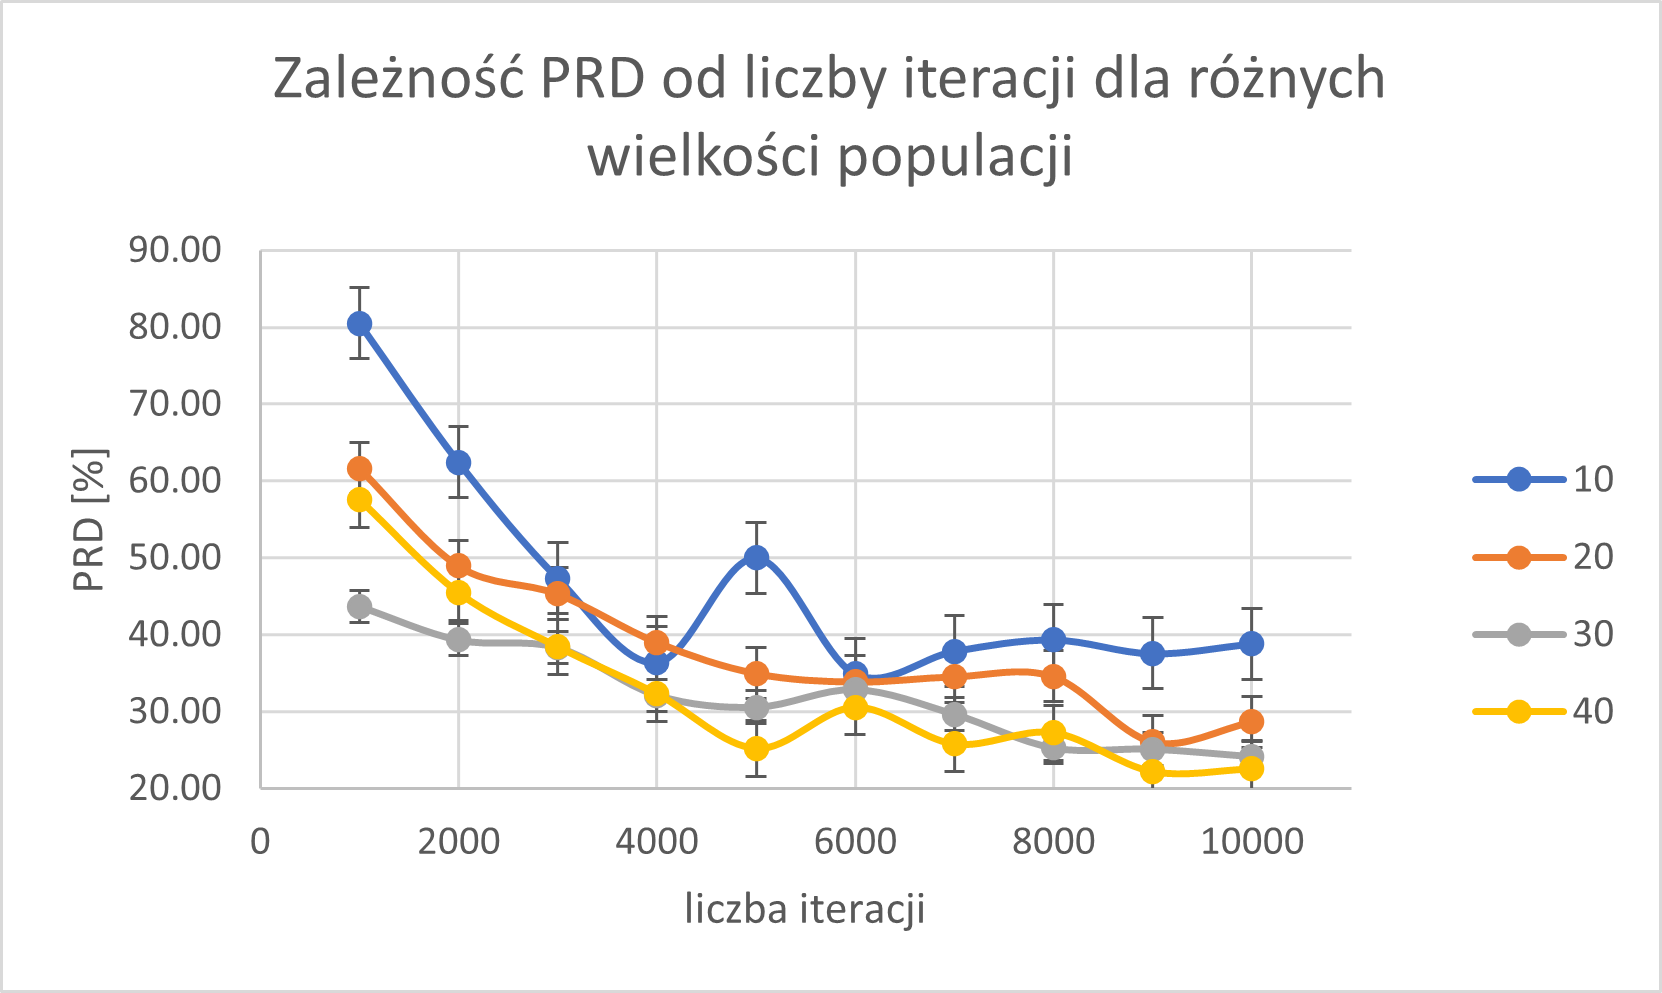
\includegraphics[scale=0.75]{chart_test_1.png}
      \centering
      \caption{Zależność PRD od liczby iteracji dla różnych wielkości populacji}
    \end{figure}
  
  Na wykresie przedstawione są średnie wartości PRD dla badanych danych. Uśrednione wartości PRD maleją logarytmicznie, wraz ze wzrostem liczby iteracji.

  \subsection{Wnioski: }
  Zgodnie z oczyekiwaniami, zwiękaszanie ilości iteracji zwiększa jakość rozwiązań jednak w okolicach 5000 iteracji zaczyna poprawa zaczyna być coraz mniejsza - zależniść nie jest liniowa, raczej logarytmiczna. Dodatkowo z wykresu można odczytać że zwiększanie rozmiaru populacji nie koniecznie zwiększa jakość rozwiązania dla jednakowej ilości iteracji.
  

